%
%
Figure \ref{fig:parameterization_compare} compares results from four physical configurations describing thermohaline mixing in MESA: the upper left panel shows results from the Brown model; the remaining three show results from the Kippenhahn prescription with $\alpha_{\text{th}}$ varying as indicated. The reduced density ratio $\log_{10} r$ is shown as a function of mass and metallicity and indicated on the color bar and grid labels.
Simulations for which our algorithm does not measure a good thermohline zone are marked colored grey and have no label; this happens at high mass and low metallicity.
%

In all cases, the most notable trend is that $\log_{10} r$ decreases along the diagonal from high masses and metallicities (upper left) to low masses and metallicities (lower right). 
There is particularly high qualitative similarity between the Brown model and Kippehahn model with $\alpha_{\text{th}} = 2$. 
The case with the lowest mixing parameterization is the Kippenhahn $\alpha_{\text{th}} = 0.1$ case, and there the span of $\log_{10} r$ values is smallest; however, there is no clear relationship between the spread of $\log_{10} r$ values observed when using the Kippehnahn prescriptions and the values of $\alpha_{\text{th}}$ adopted in each. 
We also note that, unlike in the other three cases, $\log_{10} r$ does not scale precisely monotonically with mass or [Fe/H] in the Kippenhahn $\alpha_{\text{th}} = 700$ case. 
However, the behavior of $\log_{10} r$ is broadly consistent regardless of the theoretical assumption adopted.

The overall trends of $\log_{10} r$ vs.~[Fe/H] and mass are  
%regardless of the
robust across 1D thermohaline mixing model assumptions, suggesting that $r$ may be useful as a mixing diagnostic in physical data sets. We explore its application to observations subsequently.


\begin{figure*}
    \centering
    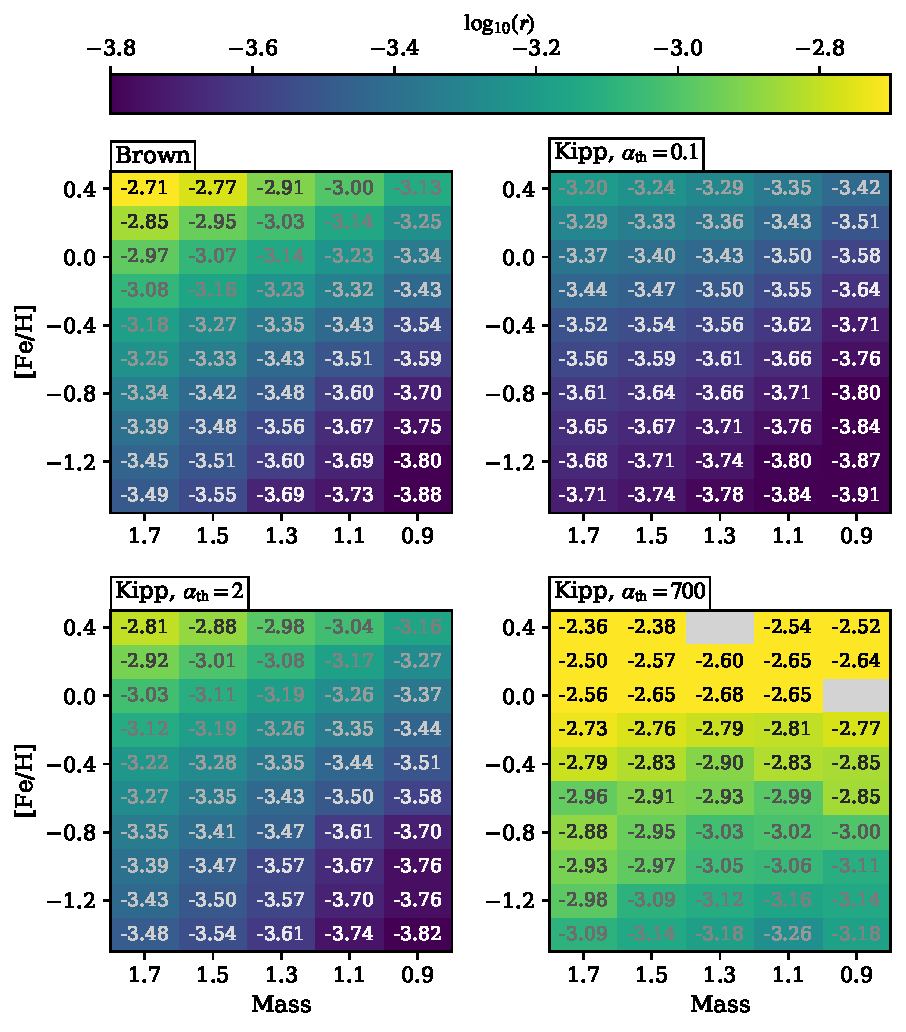
\includegraphics[width=\textwidth]{figures/mesa_spread/mesa_r_spread.pdf}
    \caption{The reduced density ratio $\log_{10} r$ is extracted as discussed in Section \ref{sec:mesa_experiment} for four grids of stellar models with differing prescriptions for thermohaline mixing. 
    Results for $\log_{10} r$ are shown as a function of stellar mass and metallicity [Fe/H], with high values of $\log_{10} r$ in brighter colors (yellow) and low values of $\log_{10} r$ in darker colors (purple). 
    The model name and mixing efficiency, $\alpha_{\text{th}}$ (where applicable) constitute the physical configuration and are indicated in the panel labels.}
    \label{fig:mesa_r_spread}
\end{figure*}